\section[cfDNA]{Cell free DNA is more than just bits and pieces}
\label{intro-sec:ctDNA}

When a cell from a multicellular organism dies, through which ever method, there will be numerous enzymes involved, which clear the debris and recycle material. This means that proteases digest proteins into amino acids, which will later be used for either building new proteins or possibly even digested further for energy production. The same happens with the DNA in the cell. However, as discussed in the previous section~\ref{intro-sec:DNA} the DNA is wrapped around histones and organised in structures called nuclesomes. These protect the DNA from being cut by DNAases by hindering the access to the DNA, similar to how they stopped the access for transcription into RNA. This then in turn leads to the DNA being cut into pieces mainly in the length of 167 base pairs (bp). 

These DNA fragments, which are called cell free DNA (cfDNA), can then be detected in bodily fluids, like blood or even stool. By analysing these fragments, non invasive tests for prenatal care have been possible, as the DNA of the foetus is detectable in the mother's blood \cite{Dan2012,Nicolaides2013}.
Similar to the process, a cancer also sheds DNA, titled circulating tumour DNA (ctDNA), when its cells die, either through intervention of the immune system or through other forcefull processes. These ctDNA fragments can also be analysed and molecular properties measured, without even knowing the exact location of the tumour. As a blood test can be routinely performed in the clinic or even a general practitioner, the monitoring of cancer progression is significantly easier and safer than through other measures. Of course, it is, similar to the prenatal test, only a proxy for the cells which are still alive, as these have not shed their DNA. Additionally, the amount of shedded DNA is highly variable between tumours, with a general higher amount for later stages, so that sometimes there is almost no ctDNA present, even though the cancer is fairly advanced \cite{Diehl2008,Schwarzenbach2011}.

\begin{figure}[ht]
\centering
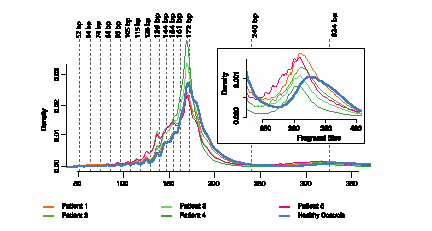
\includegraphics[width=0.9\linewidth]{Figures/intro/fragmentSizeDist}
\caption[Fragment size distribution of ctDNA]{Fragment size distribution of 5 high grade serous
ovarian carcinoma (HGSOC) patients and panel of healthy controls. The vertical dashed lines are placed on the fragment sizes between 52 and 172 bp where 10 bp periodicity is observed. The vertical lines at 240 and 324 bp show the range at which a shift in the di-nucleosomal peak occurs between HGSOC patients and healthy controls. The inset plot enlarges the density profile in the di-nucleosomal fragment length range. Figure adopted from \textcite{Markus2022}}\label{fig:ctdnaFragSize}
\end{figure}

Due to the different biological processes which lead to the release of DNA from cancer cells, in contrast to apoptosis, which is the main source for healthy cells, ctDNA has several biological differences to cfDNA. The most prominent features observed are ctDNA fragmentation size, fragment start site, and fragment ends motive. While a preferred end motive and start site are heavily correlated, selecting for cfDNA fragments of 74-155bp and 240-325bp allowed a tumour signal enrichment of at least 28\% and using all three features added another 7\% (\autoref{fig:ctdnaFragSize}, \cite{Markus2022}). 
